\subsection{Habitat Simulator and Lab- Overview}

We use the Habitat platform as a host for the EQA task. The name 'Habitat' is derived from  the notion of learning within and from an environment. Imitating our natural habitat, the Habitat platform facilitates spawning an agent in a simulated environments with the possibility of teaching the robot to preform different tasks. 

The perquisites needed to test or train an agent for a certain task in a given environment, are facilitated by a core component called  Habitat Simulator. Habitat Simulator is responsible for simulating an  environment and insinuating a robot in it. The simulator acts depending on the configurations given to it. 

The configurations are processed into commands in Habitat-lab before being passed to the simulator. Habitat lab is the second core component of the system. In addition to giving commands to the simulator, the Habitat Lab module acts as a pipeline that prepares the data-set of the corresponding task. The habitat-lab module,in other words, is the coordinator that informs the simulator of the required setting, and the data loader and processor that prepares the data for either training or testing. 

\begin{figure}[H]
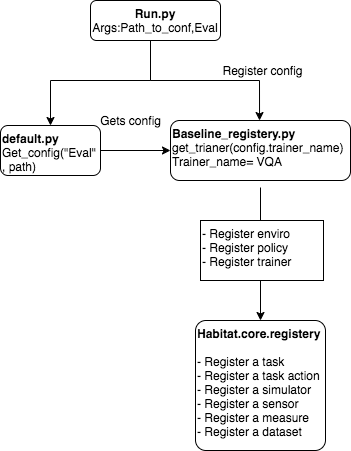
\includegraphics[scale=0.43]{images/configProcess.png}
\label{fig:configs}
\end{figure}

Figure(x) resembles a map of the code structure when the habitat lab module is initiated to preform a task. Each task has its own configurations and in this example the task is 'VQA evaluation'. As seen in the figure \ref{configs}, the module takes hierarchical steps in which each step is executed in accordance to the configuration of the given task. In the most down box of the structure we see parts of the commands directed for the simulator, such as insinuating an environment and sensors in the agent. Other commands include registering a data-set which takes part in lab module. 


Embodied question-answering is part of the tasks included within the Habitat platform. The EQA task consist of two sub tasks. The first is navigation, and the second is Visual Question-Answering. The main idea of the task is that agent needs to successfully navigate to the target object. Once the agent reaches the goal it would stop at the target location and would process the question and the visual input to answer the question. 


However, there is no available connected model that connects(Nav,VQA). The researches elaborate that the system preform poorly if the two modules put to work together and trained in reinforcement learning. Setting up the task in such a connected manner lead to distorted images and inaccurate view point of the object in question if the robots drifts off the path during navigation. "Noisy or absent views"  would confuse the question-answering model.

The current configuration for the EQA task separates the training for navigation and VQA. Imitation learning is used for navigation, and supervised learning for question-answering. the navigation is frozen when once it completes a navigational episode and is evaluated based on its steps following the shortest path to the objective. VQA model is evaluated based on the answers predicted.  

'shortest path' is used in the training sitting of both, the navigation and VQA. 'Shortest path' is a navigational path consisting of the shortest steps to take to reach a view point of where the object in question is located. With each question-answer in the EQA data-set we find one shortest path. Shortest paths are made by human workers. For navigation the system is trained on following the steps of the shortest path. For VQA the shortest path is used to capture the scene from the viewpoint at the end of the path.  

However, the navigation might go off the shortest path and seek to take more actions to reach the goal. This might lead to distorted images and inaccurate view point of the object in question. "Noisy or absent views"  would confuse the question-answering model.

The vision-language modalities are fine-tuned differently for navigation and QA. Navigation and VQA employ the vision and language modalities provided in the platform. However, each one of them use the two modalities with different configurations, such as the number of decoders for vision and  the times that the language encoder is used.  


\subsection{vision}

The vision of the system relies on egocentric 224x224 RGB images processed in CNN. The CNN encoding has the functionality of a “multi-task pixel-to-pixel prediction framework,” which consists of 4 {5x5 Conv, BatchNorm, ReLU, 2x2 Max-Pool blocks}, and they produce a fixed-size representation.“The range of depth values for every pixel lies in the range r0, 1s, and the segmentation is done over 191 classes”(p.11). (page,6). 

It  is possible to train the encoder-decoder on generating  three sensory information. The three decoders, which can also be referred to as sensors take the functionality of: 1) RGB reconstruction, 2) semantic segmentation, and 3) depth estimation. The latter sensors are used to obtain “object attributes (i.e., colors and textures), semantics (i.e., object categories), and environmental geometry (i.e., depth).” . 

In the baseline models, different tasks take different sensors.Not all the above-mentioned sensors are used in all the baseline tasks. Since navigation and VQA are trained and evaluated separately, we refer to them as separate "tasks". The two tasks in EQA take the following sensors: 

{Navigation}:  "depth" and "RGB". Depth sensor is essential for the agent's capability to navigate. With depth sensor it could estimate distances and avoid colliding with obstacles.  

{VQA}: The existent baseline VQA model uses the visual information with "RGB" data only. (No reason mentioned to why the other sensors are not used in the question-answering baseline module).  


\subsection{language model}

The language models is a 2-layer LSTM with 128d hidden layers. The language model's role is to encode the questions and produce a representation. The language-encoder is trained differently for the navigation and VQA. The encoder learns to focus on different strings for each task. Some words in the question can be crucial for executing one of the tasks while less useful for the other task. An example of a question, cited from the EQA paper, " ‘What color is the chair in the kitchen?’, ‘color’ is irrelevant for navigation and ‘kitchen’ matters little for question answering (once in the kitchen) "

%Hence- current hidden-state h_{t} and the current action are only %updated in the planner: 
%
%The controller executes the action  a_{t+1}. It takes then the 
%
%Hence, h_{t-1} and a_{t-1} carry no information at the 0 timestep %since no encoding or action been outputed by the planner at the 0 %step; Thus they are more like an initiation in this example.  
%
%The planner passes the current action a_{t} and the current hidden %state h_{t} to the controller 
%



\subsection{Data and Data-sets}

 Our method of generating questions is largely related to the structure of the data-sets in the initial EQA paper\cite{embodiedqa}. Understanding each part of the data-sets and their structure would give an insight into the work flow of generating questions to the task. In this section we elaborate on the source of the data-sets, their content, and our methods in processing the data. 
 
The data-sets consist of two parts. One is a 3D indoor enviroments, and the other is a question-answering data-set. The 3D enviroments are constructed images that assimilate real indoor enviroments. The 3D Scenes and the QA dataset mentioned in \cite{embodiedqa}, are called SUNCG(3D houses) and "EQA V1" (QA). The EQA V1 is a synthetic dataset generated automatically, and constructed based on the setting of the 3D houses in SUNCG. 

SUNCG is no longer available. \cite{embodiedqa} changed the SUNCG 3D setting to MatterPort 3D (MP3D). MatterPort 3D is a reconstruction of 3D houses in (SUNCG) scene dataset. The latter also implies that the inital "EQA V1" is not applicable for MP3D. 

The new QA dataset for Matterport 3D is available but not the code that generated it. The EQA-mp3d v1 is also a synthetic dataset generated automatically and can be found at this footnote reference \footnote{https://github.com/facebookresearch/habitat-lab}. For generating  questions for SUNCG, a code published at this reference\footnote{https://github.com/facebookresearch/EmbodiedQA}. However, there is no code for generating QA for MP3D. 
 
A few of the differences between the question dataset for SUNCG (EQA-SUNCG) and MP3D(EQA-MP3d) are mentioned in \cite{eqa_matterport}. However, not in all the information in  \cite{eqa_matterport} seems to match with EQA-MP3D that we have. In  \cite{eqa_matterport} page(4) it's stated that the number of scene used from MP3D is 76. The dataset we downloaded from "facebookai/habitat" repo on github uses a total 67 scene of 90 scenes available in MatterPort3D. 57 of the 67 scenes are used for questions in the train-set and 10 in the the enviroment. Note that the latter implies that the robot is tested on different scenes from the scenes it has been trained in. 

We refer to each question-sample in the EQA data-set as an "Episode". Each question is an episode, because the sample contains also, on the topic of the question-info, geometric information and shortest paths. Each episode is applicable for navigation and VQA, and can be run for each task separately. 

The EQA-v1 dataset consists of 1950 validation sets and 11000 training questions.

\subsubsection{Scene Data-set and semantic annotations}



(restructuring is required-- more precision) (examples to rephrase-- why do we need the location in global coordinates and why the camera views are also important)

The MP3D dataset provide 90 segmented houses with their semantic annotation. The semantic annotation is segmented based on the structure of the house. The segments consists of house levels(floors), to regions(rooms), and objects. The annotation is organized accordingly, such as that an object is annotated and indexed in relation to room and the floor its located in. 

For example, the annotation of a house begins with the first level in it, followed by the rooms and objects in each room as: house 1 [{level1:room1[bedroom]:(obj1:bed,obj2:..),room2:(obj..)},, {level2:......} ]  

Each semantic annotation include geometric information. The geometric information consist of elements as location of an object, region or level, defined by their center in a world coordinate system. Other information is the size of the entity given its radius from its starting location (center).   

The camera views of the scenes are globally oriented \cite{Matterport3D}(p3). A way to allocate an object is to find its location in a accordance to global coordinates. Let's say the global coordinates start from the center of a house where the center of the house is (0,0,0) on the (x,y,z); and let's say all the objects are spawned through out the house's (x,y,z) axis where each objects location is defined by its distance to the house center. When annotated, the objects are viewed through a camera. The description of their geometric location, thus, should consider the view-postion of the camera. 

\begin{figure}[H]
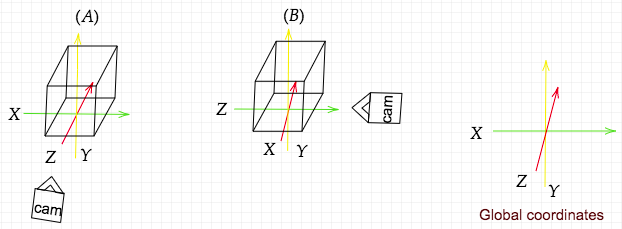
\includegraphics[scale=0.53]{images/campos.png}
\label{campos}
\end{figure}

In graph (A) in \ref{campos}, we see that the camera-view of coordinates align with the global coordinates.The (x,y,z) that go through each object in graph(A) and graph (B) are the view of the axis in reference to the camera. However, if the camera is positioned to the right of the object from our view, as in graph (B), then we say that the camera view of coordinates is not aligned with the global view. We notice in graph (B) that from the camera view, the "global X" is "Y" and vice versa.

Some geometric calculations cannot be preformed if the location measurements are not relative to each other. For example, if we want to calculate the distance between objects the locations must be consistent with one reference point. The camera position is changing and if the location of an object is referenced by the camera's position then we would get locations relative to the changing position of the camera in a time-span. 

To globalize the orientation of the view, measures such as top-down view of a map, or calculating the rotation of the camera from the global center. While the global locations are crucial for measuring the distance, other point-views are also crucial for other purposes. There are three essential coordinate systems to know when working in a 3D environments: 

\textbf{1. World coordinates}(global):  World coordinates(global): The coordinate system that starts at the center of the world; a house in our example. The center of an object in this coordinate system, is then decided by its distance to the center of the world. 

\textbf{camera-view coordinates:} The coordinates from the camera's views. The center of this coordinate system is the position of the camera. The center of the object in this world is defined by its distance to the camera. 

\textbf{3. Local view:} The center of the local view is the object itself. 

The center of all these views is (0,0,0). We described above that the world coordinate system allows us to measure distance between objects in a world map. The camera view is useful if a robot is expected to navigate an environment and describe spatial relations between objects such as "next to", "above". The local view could tell about the size of an object. In particular, the (x,y,z) from a local point of view tell about how far the object stretches from its center where the center is (0,0,0). The local view can be referred to as "radius". 

MatterPort 3D provide the views decribed above. We discuss in more detailed the usage of the object's location in global coordinates and the local view in details in the implementation part.  

\paragraph{Processing geometric data- Methods}

\begin{figure}[H]
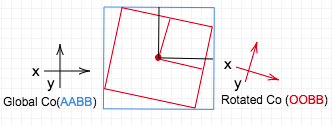
\includegraphics[scale=0.5]{images/A-OB.png}
\label{}
\end{figure}


The geometric information can be classified into two main categories. In a 3D environment we can imagine each object having  a labelling box rotated and oriented around its shape, and other box that bounds the first box with the global coordinates. In figure(X) we see a demonstration of the two boxes in 2d squares. The red box, that is meant to surround an object, is referred to as 'Object Oriented Bounding Box' (OOBB). The coordinates of the OOBB are rotated with rotation of the object (rotated in accordance to the local view). The blue box is referred to as 'Axis Aligned Bounding box'(AABB). The axis of AABB are aligned with global coordinates. 

We extract and save one specific information type of each box. The feature we take is the "radii", or else can be referred to as half-extents. The half-extents (radius) can be helpful in representing the object in different ways.  

We use the radius of the OOBB box to calculate the size of an object. The volume of OOBB gives more precise estimation of the size of the object, as the box is more enclosed around the object.

We use the radius of AABB box to measure the distance of an object to other objects. We can measure the distance between objects in an environment by the distance between their centers. More precise measurements would be to measure the edges or the corners of the object. We get the corners by measuring how far the box stretches(given by radius) from the center.  

Important to mention that we locate entities on a map with coordinate points that are positioned in accordance to one coordinate system (grounded in a the global map). Otherwise the numbers that represent positions would be in-indicative of points in the global view . It is for the latter reasons, the centers (located globally) are helpful to measuring distance-- because they are located on the same coordinate basis.  

The AABB box, provide a straightforward estimation of the positions of the object's shape in the global map. The local view of the AABBs are aligned with world coordinates, therefore allocating its corners globally would only require an estimation of how its radius(given in alliance with world coordinates) stretches from the center.

True that the OOBB corners are better representatives of the objects corners, however, locating the oobb corners in the world map is not simply done by measuring how its radius stretches from the center in the direction of  the global axis as in AABB. The radius of the OOBB is given along its local view axis(its rotation), meanwhile the center point is given in the world axis. Thus, locating the positions of the OOBB, using the same radius-length measure, would require adjusting the radius to the direction of its rotation. Therefore, the global-alignment characteristic of the aabb provides a direct way to locating its edges.  


The corners of the OOBB would be the most precise representation of the corners of an object. 



\subsubsection{EQA (Task Dataset)}

(More information to include-- 1. How they filter out questions based on entropy, and how they filter out objects based on size..2.How many unique question there is. 3. Explain more thoroughly how the singleton(object,room) works) 

The question-answer data-set contains three types of questions.
Each question in the detest is a function that can be executed in the environment to give an answer. More in section (3.2)
\begin{figure}[H]

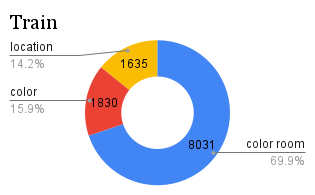
\includegraphics[scale=0.45]{images/Train.png}
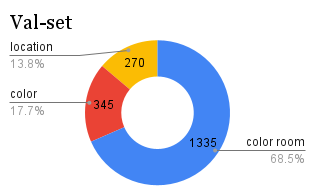
\includegraphics[scale=0.45]{images/Val-set.png}
\end{figure}

%\begin{figure}
%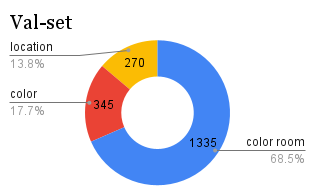
\includegraphics[scale=0.45]{images/Val-set.png}
%\end{figure}


(To include the number of unique questions here )
There is a total 11496 questions in the train split and 1950 questions in the val split. As seen in figure (5),in the train split there are 1830 questions "color" type, 8031 of "color room"  and "1635" of location type. For the validation split there are 1335 "color room" questions, 345 "color" questions, and 270 "location" questions. 



Each question-type is generated in a string template.The templates are as the following:

\textbf{- color room} template: "what color is <obj> in  <room>?": In these questions the agent needs to find the room in question and look for the object and answer the question. For the agent's to be successful at reaching its target, it needs to know the difference between rooms, and objects, as by implicitly recognizing that a certain room is a living-room, not a bathroom and such.  

\textbf{- color} template: "what color is <obj>". The difference between "color" type and "color room" is that no room is specified in the "color" type of question. In "color" type the agent needs to figure out where to look by itself. For example, "what color is the fridge?", the robot needs to implicitly figure that the fridges are usually in the kitchen and navigate to the kitchen to answer the question. In other cases, the object could be in the vicinity of the robot's starting point, so that it all it needs to do is to look around. 

\textbf{- location} template: "What <room> is the <obj> located in". 

\paragraph{Querable objects and rooms}

The questions ask about 50 unique objects. \cite{embodiedqa} in (page 4) describe the process of object and room selection for question generation.The following quoted from (page 4): 

"select(objects)->singleton(objects)->query(location)"

The above represents the steps taken for finding object and location to fill in the questions template. select(objects) is a function that collects all the objects in the house. singleton(objects), filter out an object that occurs only once in the house; query(location) finds the location of the object.However, this applies to the old dataset in SUNCG.

In EQA-MP3D, the object in question is not unique to the house but to the room. The latter means that for an object to be selected for a question, there need to be only one instance of that object existent in the room. The reason for this is to avoid ambiguity, and not to confuse the agent if there happen to be more instances of the same object in the room. 

we observe that all the objects that the robot is asked about in testing have occurred in the training questions. While it has been mentioned earlier that the robot is tested in different scenes from the scenes it was trained on, similar objects from the training co-occur in the testing. The latter means, in particular, that the robot is unfamiliar to the test scenes but familiar with all the objects that are being asked about in the test. This information is also stated in \cite{eqa_matterport}. 


\paragraph{Structure}

\begin{figure}[H]
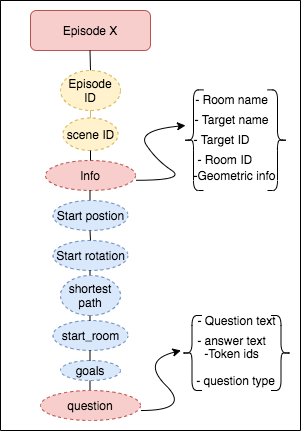
\includegraphics[scale=0.5]{images/episode1.png}
\label{fig:episode}
\caption{}
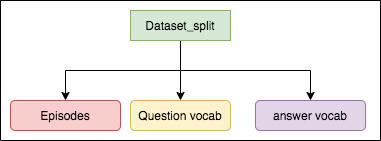
\includegraphics[scale=0.5]{images/datasplit1.png}
\label{fig:datasplit}
\caption{}
\end{figure}

In figure (x) we see the top structure of the val and test. \textit{Episodes} refer to each question-function in the data-set split. \textit{Question vocab} and \textit{answer vocab} contain the same elements as dictionary keys. The elements are: [word list,stoi,itos,num vocab,pad token].

"Question vocab" and "answer vocab" in the "train" and "val" are identical to each other. When using each split of the dataset, the answer-tokens that are considered are the ones contained within the episodes instead of the word-lists mentioned above. 

Each question-sample is an episode that consist of multiple layer information. The structure of one episode of all the "episodes" is as seen in figure(x). We describe the elements of an episode in the following:  

\textbf{House ID}: The house ID given by the house ids in MatterPort3D.
\textbf{Episode ID}: The episode index in the range of the split's length. \hspace{1.5cm}
\textbf{Info}: This element contains all the information about the the object and room in a question. The information is structured as such: 

Information about the traget-object is the first layer within "info": 

\textit{centroid}: The center of the object's box in the global coordinates. Box is the area that labels  the object. When the center is globally oriented we would refer to this center and box as Axis-aligned bounding box(AABB), which means that (x,y,z) axis of the center are aligned with global coordinates. 

\textit{radi}: It tells how far the box (object) stretches from its center one direction of each axis. The value of radii is relative to the object itself (from the local view), where the center is zero. If we have, for example a radi of (2,1,4), this means that the object's box stretches +2 and -2 from the center on the x axis. The boundaries of the object's box relative to itself is referred to as object oriented bounding box (OOB). 

\textit{level}: at which level-floor of the house  is the object located in. 

\textit{room-id}, \textit{room name},\textit{obj Id},\textit{room name} : Room ID, room name and object ID as given by semantic annotation in  Matterport3D. Many of the objects are re-named, mostly names in hyponymes changed to hypernym category such as: round-sofa, l-shaped sofa changed to their hypernym category "sofa". 

The second layer is information about the room: 

Information about the room is similar to the type of information given for the objects. Th information is \textit{floor-level}, \textit{room-id}, \textit{room name},

Final layer consist of a "question-meta" which includes the color of the object. This section also includes question-entropy ..... 

The elements that are marked in blue in figure(x) are navigation-related material. 

\textbf{start position}: The start positions are all unique. For each unique question in the data set there is fifteen different starting position. 

\textbf{rotations}: This is the rotations that the agent have to do while navigating. It stands as supplementary information for the shortest path 

\textbf{goals}: Goals are the destinations that the agent should reach in navigation. The goals stand for the possible view points from where the the target object can be looked at by the robot. Each view point consist of geometric position and the rotation toward the target object respective to the position. 

%\begin{figure}
%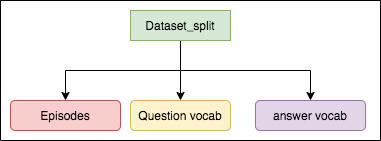
\includegraphics[scale=0.5]{images/datasplit1.png}
%\end{figure}



\paragraph{expirement}


The idea is to extend the question asked for the agent. The two types of questions are size and spatial. The process of question extension includes using information from the initial EQA-v1  dataset, which consists of color, color-room, and location questions. Each question sample has a target object with corresponded information as object ID, room ID, Scene ID, question(token-ids and text), and shortest path. We pick the object and the room ID for every question sample to extract the rest of the information about the other things in the room. The extracted information is the volumes of the objects and the 


